\subsection{Calcul de la hauteur d'eau à propager}
La première étape consiste à calculer la quantité d'eau présente à la surface de la SU. Si une fonction préalablement appelée par le modèle produit de l'exfiltration, alors la fonction calcule la lame d'eau par l'équation suivante :

\begin{equation}
\label{height}
H = R + \left(\frac{Q_e\times \Delta t}{A}\right)
\end{equation}


où $H$ est la lame d'eau présente à la surface du sol ($m$), $R$ est la hauteur d'eau ruissellante ($m$) générée par la fonction de production, $Q_e$ est le débit d'exfiltration ($m\up3/s$), $A$ est la surface de la SU ($m\up2$) et $\Delta t$ est le pas de temps de simulation ($s$).\\

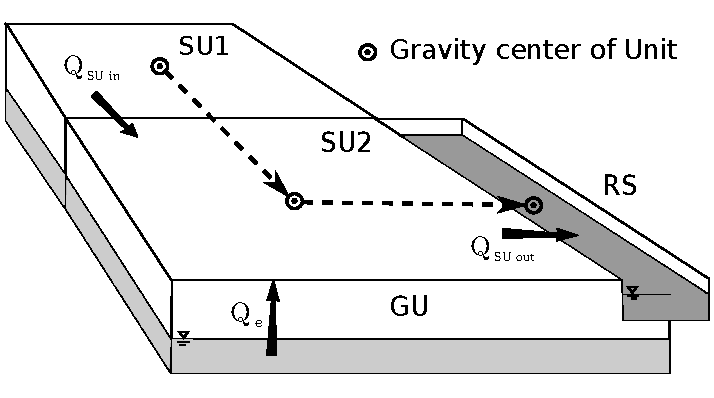
\includegraphics[width=8cm]{common/Schema_GU_RS_SU_Hayami_SU.pdf}

Le débit d'exfiltration $Q_e$ peut être notamment produit par la fonction ``Ecoulement de subsurface''.\\


\subsection{Propagation selon le noyau d'Hayami}
Ensuite, la lame d'eau calculée précédemment est propagée entre le centre de gravité de l'unité hydrologique sur laquelle est effectué le calcul et celui de l'unité située en aval. Cette unité peut être une unité de surface SU ou un tronçon RS selon la topologie. Le calcul de propagation de l'onde est ainsi effectué selon l'ordre de Straler, depuis les SU amont jusqu'au SU aval.\\

La propagation est réalisée selon le modèle de l'onde diffusante :

\begin{equation}
\frac{\delta Q}{\delta t} = -C \times \frac{\delta Q}{\delta x} + D \delta \frac{\delta \up2 Q}{\delta x\up2}
\end{equation}




Les paramètres de célérité et de diffusivité de l'onde étant considérés constants dans le temps, l'équation de l'onde diffusante peut être résolue de façon analytique par la méthode d'Hayami \cite{Moussa1996}. La méthode consiste à convoluer la hauteur d'eau d'entrée en résolvant l'équation suivante :

\begin{equation}
\begin{array}{l}
Q_{SU}(t) = \frac{d}{2\times (\pi \times D)\up{1/2}} \times exp ^{\frac{C \times d}{2 \times D}}
\\
\ \ \ \ \ \ \ \ \times \int_0^t H(t-\tau)\times A \times \frac{ exp ^{\frac{C\times d \times}{4\times D} \times \left(\frac{d}{C \times \tau} + \frac{C \times \tau}{d} \right)}}{\tau \up{3/2}} \delta \tau
\end{array}
\end{equation}




où $Q_{SU}(t)$ est le débit de ruissellement produit par la SU au temps $t$ ($m\up3/s$), $d$ est la distance entre les centres de gravité des deux unités connectées ($m$), $D$ est la diffusivité de l'onde ($m\up2/s$), $C$ est la célérité de l'onde ($m/s$), et $A$ est la surface de la SU ($m\up2$).\\

Le terme $H(t-\tau)$ est la hauteur d'eau présente à la surface de la SU calculée dans l'équation \ref{height}. Cette hauteur d'eau est convoluée avec le ``noyau d'Hayami'' $K(t)$ qui est exprimé ainsi :

\begin{equation}
K(t) = \frac{d}{2 \times (\pi D)^{\frac{1}{2}}} \times \frac{\text{exp}^{\frac{Cd}{4D} \times \left(2-\frac{d}{Ct}- \frac{Ct}{d} \right) } }{t^{\frac{3}{2}}}
\end{equation}




L'opération de convolution peut être schématisée de la façon suivante :

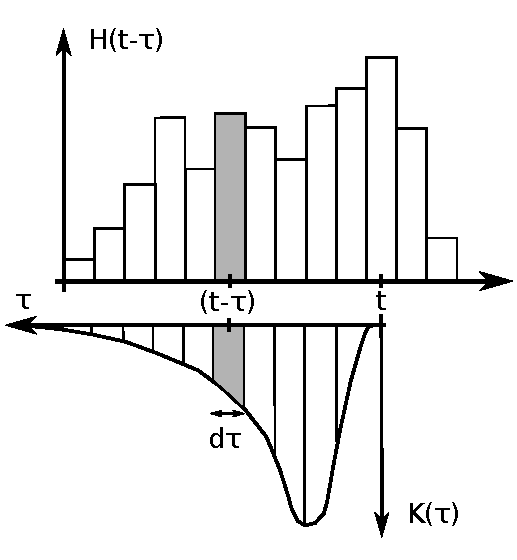
\includegraphics[width=8cm]{common/Convolution_HayamiSU.pdf}

$\tau$ est un opérateur de convolution interne à la fonction. La fonction réalise un balayage temporel du noyau d'Hayami au pas de temps de simulation $\delta \tau$ et sur une durée déterminée par le paramètre $MaxSteps$ ($-$). Ainsi, le noyau d'Hayami est défini sur une durée égale à $MaxSteps.\Delta t$. Par conséquent, ce paramètre doit être ajusté en fonction de la forme du noyau d'Hayami et du pas de temps de simulation. Plus ce paramètre sera grand, meilleure sera la définition du noyau d'Hayami. D'autre part, plus le pas de temps sera petit, meilleure sera la résolution du noyau d'Hayami. Pour obtenir une paramétrisation optimale, il est conseillé d'initialiser la valeur de $MaxSteps$ à une valeur élevée et de la diminuer tant que cela n'impacte pas les résultats.\\

Les deux paramètres $C$ et $D$ du modèle peuvent être reliés à la pente et à la rugosité de l'unité de surface en utilisant une relation de type Manning-Strickler.

\begin{equation}
C=C_u\times \sqrt{\frac{\beta}{\beta_m}}\times \frac{n_m}{n} \ \ \ \ \ et \ \ \ \ \ D=D_u\times \frac{\beta}{\beta_m} \times \frac{n_m}{n}
\end{equation}


où $C_u$ est la célérité moyenne sur l'ensemble des SU ($m/s$), $\beta$ est la pente de la SU sur laquelle est effectué le calcul ($m/m$),  $\beta_m$ est la pente moyenne de l'ensemble des SU ($m/m$), $n$ est le coefficient de rugosité de la SU ($s/m\up{1/3}$), $n_m$ est le coefficient de rugosité moyen sur l'ensemble des SU ($s/m\up{1/3}$) et $D_u$ est la diffusivité moyenne sur l'ensemble des SU ($m\up2/s$). Ce calcul est effectué une seule fois en début de calcul.\\

La diffusivité et la célérité vont déterminer la forme de l'hydrogramme unitaire d'Hayami comme présenté sur la figure suivante :

\begin{equation}
w = \frac{L}{D} \ \ \ \ \ z = \frac{C.L}{4.D}
\end{equation}



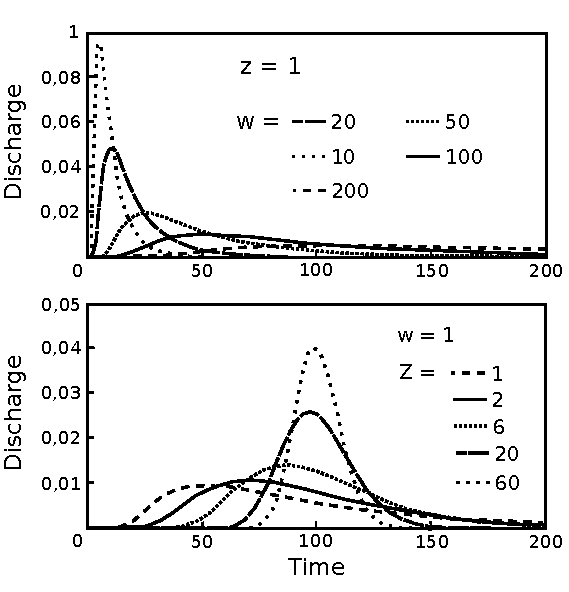
\includegraphics[width=8cm]{common/Graphique_noyau_Hayami.pdf}

Des exemples d'application et de paramétrisation de ce modèle sont disponibles dans la thèse de Chahinian \cite{Chahinian2004} et dans les travaux de Moussa et al. \cite{Moussa2002}.\\
